\section{Introduction}
\label{cha:intro}

The 0--1 loss objective for binary classifiers --- minimize the number
of misclassifications --- is known to be robust to outliers.
Unfortunately, it is NP--hard to optimize directly
\cite{Feldman,nphard} and thus most work has sought alternative losses
with better computational guarantees.  While hinge loss used in
SVMs~\cite{Vapnik} and log loss used in logistic regression may be
viewed as convex surrogates of the 0--1 loss that are computationally
efficient to globally optimize~\cite{Bartlett}, such convex surrogate
losses lead to the problem of outliers~\cite{wu07,outliers,Ding} as
shown in Figure~\ref{fig:svm_failure}.

%%%%%%%%%%%%%%%%%%%%%%%%%%%%%%%%%%%%%%%%%%%%%%%%%%%%%%%%%%%%%%%%%%%%
\begin{figure}[t!]
\vspace{-4mm}
\hspace{-3mm} 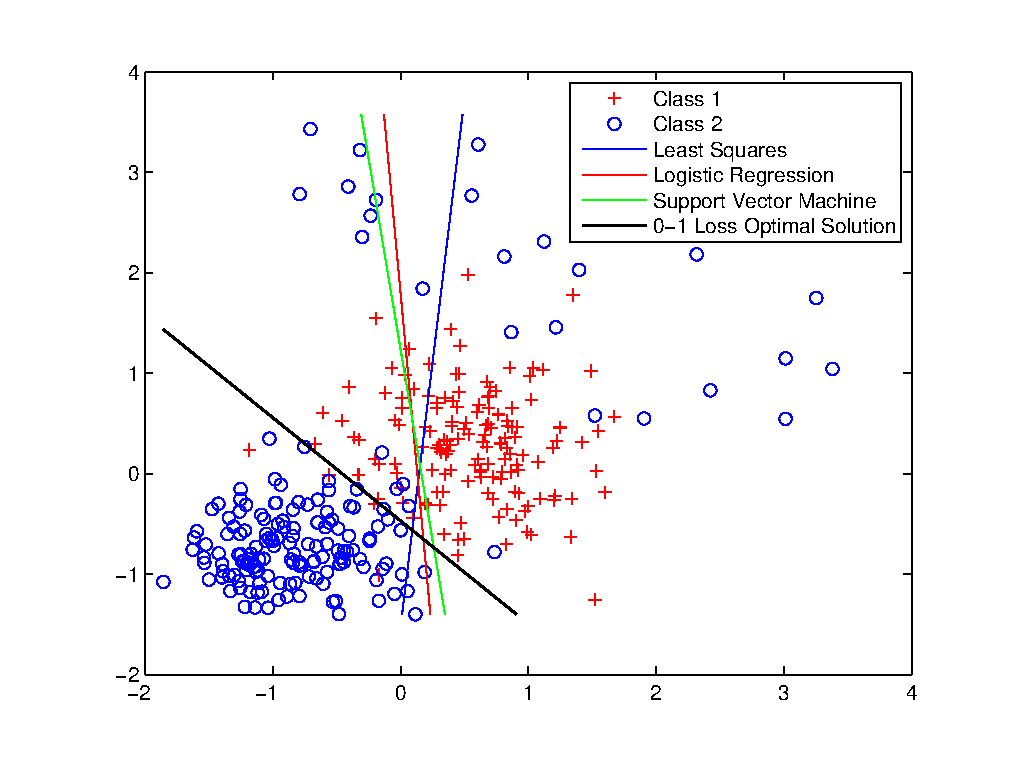
\includegraphics[width=0.50\textwidth]{images/fig11_svm_failure2.eps}
\vspace{-9mm}
\caption{ \footnotesize Training data consisting of 300 points of two
  classes, 10\% of which are outliers.  All convex losses (least
  squares, logistic regression, SVM) are skewed by the outliers and
  their decision boundaries make $\geq$ 61 classification errors,
  whereas the optimal 0--1 loss solution makes 39 errors with a decision
  boundary that is robust to the outliers.}
\label{fig:svm_failure}
\vspace{-4mm}
\end{figure}
%%%%%%%%%%%%%%%%%%%%%%%%%%%%%%%%%%%%%%%%%%%%%%%%%%%%%%%%%%%%%%%%%%%%

Given the outlier robustness properties of 0--1 loss, we explore a
variety of practical algorithms for directly optimizing it and
contribute the following novel optimization techniques targeted
specifically for 0--1 loss:
%\begin{itemize}
%\item 

% In a linear XADD, all decisions can be seen as data points and
% hence maybe can use this convex hull technique to identify child
% decisions whose branches can be pruned -- but how is this different
% from the current pruning method?
\noindent\emph{Branch and bound:} We show this staple of search in the
optimization literature proves effective with good initialization (via
the SVM solution) plus informed decision ordering heuristics and a
forward-checking technique for pruning implied decisions within the
convex hull of existing decisions; this leads to an \emph{optimal}
0--1 loss solution for hundreds of data points.
%\item 

\noindent\emph{Combinatorial search:} We exploit the fact that there
are only a finite number of equivalence classes of separating
hyperplanes that can have different losses and propose both
prioritized systematic and heuristic search through combinations of
data points that define these equivalence classes.  While systematic
combinatorial search yields efficient optimal solutions on low
dimensional problems, heuristic combinatorial search offers excellent
approximations and scalability.
%\item 

\noindent\emph{Smooth, differentiable relaxations of 0--1 loss:} We
relax the 0--1 loss to a smooth, differentiable function that can
arbitrarily approximate the original 0--1 loss via a smoothness
constant.  We then provide an iteratively unrelaxed coordinate descent
approach for gradient optimization of this smoothed loss along with
techniques for escaping local optima.  This yields solutions
comparable to the combinatorial search approximation, while running
two orders of magnitude faster.
%\end{itemize}

Empirically, we compare our proposed algorithms to logistic
regression, SVM, and the Bayes point machine (a approximate Bayesian
approach with connections to the 0--1 loss) showing that the proposed
0--1 loss optimization algorithms perform at least comparably and
offer a clear advantage in the presence of outliers.  

%To this end, we believe this work reiterates the importance of 0--1
%loss and its robustness properties while challenging the notion that
%it is difficult to directly optimize.
